\documentclass[conference]{IEEEtran}
\IEEEoverridecommandlockouts
\usepackage[utf8]{inputenc}
\usepackage[T1]{fontenc}
\usepackage[brazilian]{babel}
\usepackage{cite}
\usepackage{amsmath,amssymb,amsfonts}
\usepackage{graphicx}
\usepackage{textcomp}
\usepackage{xcolor}
\usepackage{booktabs}
\usepackage{array}
\usepackage{url}
\usepackage{balance}
\usepackage[hidelinks]{hyperref}
\renewcommand{\IEEEkeywordsname}{Palavras-chave}
% Floats posicionados junto ao texto que os cita, com espaçamento fixo
\setlength{\intextsep}{10pt plus 2pt minus 2pt}
\setlength{\textfloatsep}{12pt plus 2pt minus 2pt}
\def\BibTeX{{\rm B\kern-.05em{\sc i\kern-.025em b}\kern-.08em
    T\kern-.1667em\lower.7ex\hbox{E}\kern-.125emX}}

\begin{document}

\title{Efeito da Filtragem por Correlação no Reconhecimento de Atividades Humanas com Classificadores Clássicos}

\author{\IEEEauthorblockN{Samuel Prado Costa}
\IEEEauthorblockA{\textit{Engenharia de Computação} \\
\textit{Centro Universitário Hermínio Ometto (FHO)}\\
Araras, Brasil \\
RA: 115116}
\and
\IEEEauthorblockN{Isaac Loureiro Eigenheer}
\IEEEauthorblockA{\textit{Engenharia de Computação} \\
\textit{Centro Universitário Hermínio Ometto (FHO)}\\
Araras, Brasil \\
RA: 115095}}

\maketitle

\begin{abstract}
Atributos extraídos de sinais inerciais costumam ser numerosos e redundantes. Este trabalho avalia o efeito de uma filtragem por correlação de Pearson ($|r|\geq0{,}95$) no reconhecimento de seis atividades humanas com dados de smartphone da base UCI-HAR. A partir dos sinais brutos, foram extraídos 344 atributos de tempo, frequência e multieixo, e cinco classificadores clássicos --- Extra Trees, Random Forest, LightGBM, SVM e KNN --- foram comparados com e sem a filtragem, em validação cruzada de cinco \textit{folds} agrupados por participante. O filtro, ajustado apenas no treino, reteve em média 191,6 atributos (redução de 44,3\%). O LightGBM obteve o maior F1 macro (95,08\% $\pm$ 2,12 com filtro; 95,04\% sem filtro) e teve o tempo de treinamento reduzido em 43\%. A filtragem aumentou o F1 macro do Extra Trees (+1,03 p.p., com ganho nos cinco \textit{folds}) e do Random Forest (+0,52 p.p.), mas reduziu o do SVM ($-$0,44 p.p.) e o do KNN ($-$1,24 p.p.), com perdas em todos os \textit{folds}, concentradas nas posturas estáticas. A análise de sensibilidade mostrou que os modelos de árvores mantêm o desempenho até o limiar de 0,80 (98 atributos), enquanto SVM e KNN pioram à medida que mais atributos são removidos. Os resultados indicam que a filtragem por correlação é útil para reduzir o custo de comitês de árvores, mas não deve ser aplicada sem verificação a classificadores baseados em distância.
\end{abstract}

\begin{IEEEkeywords}
Reconhecimento de atividades humanas, sensores inerciais, aprendizado de máquina, seleção de atributos, correlação de Pearson.
\end{IEEEkeywords}


\section{Introdução}
O reconhecimento de atividades humanas (\textit{Human Activity Recognition}, HAR) consiste em inferir, a partir de sinais de sensores, o que uma pessoa está fazendo: caminhar, subir escadas, permanecer sentada ou deitada, entre outras atividades. Smartphones e dispositivos vestíveis possuem acelerômetros e giroscópios de baixo custo, o que torna possível o monitoramento contínuo e não intrusivo em aplicações de saúde, assistência a idosos, reabilitação e esporte \cite{Lara2013,Bulling2014}.

Em abordagens de aprendizado de máquina clássico, cada janela de sinal é convertida em um vetor de atributos calculados no domínio do tempo e da frequência, que alimenta um classificador supervisionado \cite{Bulling2014}. Esse processo costuma gerar centenas de atributos, muitos deles redundantes: média, mediana e RMS de um mesmo canal, ou a energia total e a variância, tendem a apresentar correlação muito alta. A redundância aumenta o custo de extração e de treinamento e pode prejudicar classificadores baseados em distância, nos quais cada coordenada contribui igualmente para a medida de similaridade \cite{Guyon2003}. Por outro lado, descartar atributos pode eliminar informação útil. Saber se a remoção de atributos correlacionados compensa, e para quais classificadores, é relevante para projetar sistemas de HAR mais leves, especialmente em dispositivos com recursos limitados.

O \textbf{objetivo geral} deste trabalho é avaliar o efeito de uma filtragem de atributos por correlação de Pearson sobre o desempenho de cinco classificadores clássicos no reconhecimento de atividades humanas com dados de smartphone. Os \textbf{objetivos específicos} são: (i) implementar um \textit{pipeline} reprodutível de extração de atributos a partir dos sinais inerciais brutos da base UCI-HAR \cite{UCI-HAR}; (ii) comparar Extra Trees, Random Forest, LightGBM, SVM e KNN com e sem a filtragem, sob validação cruzada agrupada por participante; (iii) analisar a sensibilidade dos resultados ao limiar de correlação; e (iv) quantificar a redução da dimensionalidade e do tempo de treinamento e inferência. Todo o código, os resultados por \textit{fold} e este artigo estão disponíveis publicamente \cite{Repositorio}.

O restante do artigo está organizado da seguinte forma: a Seção~\ref{sec:relacionados} discute os trabalhos relacionados; a Seção~\ref{sec:metodologia} descreve a base de dados, a extração e a seleção de atributos, os classificadores e o protocolo de validação; a Seção~\ref{sec:resultados} apresenta e discute os resultados; e a Seção~\ref{sec:conclusao} apresenta as conclusões, limitações e trabalhos futuros.

\section{Trabalhos Relacionados}
\label{sec:relacionados}
Lara e Labrador \cite{Lara2013} revisam sistemas de HAR com sensores vestíveis e descrevem a cadeia típica de processamento: aquisição, segmentação em janelas, extração de atributos estatísticos e espectrais e classificação. Os autores apontam árvores de decisão, SVM e KNN entre os classificadores mais usados e destacam que a escolha dos atributos influencia tanto a acurácia quanto o custo computacional. Bulling et al. \cite{Bulling2014} apresentam um tutorial dessa cadeia e enfatizam que o protocolo de avaliação deve refletir o uso pretendido, por exemplo testando o sistema em pessoas que não participaram do treinamento.

Kwapisz et al. \cite{Kwapisz2011} usaram apenas o acelerômetro de um celular no bolso e 43 atributos simples por janela de 10~s para reconhecer seis atividades com árvores de decisão, regressão logística e outros classificadores. O trabalho mostrou que atributos de baixo custo já distinguem bem atividades de locomoção, mas que subir e descer escadas são frequentemente confundidos. Anguita et al. \cite{Anguita2013} publicaram a base UCI-HAR, com acelerômetro e giroscópio de um smartphone na cintura, e um conjunto oficial de 561 atributos. Com um SVM, relataram acurácia de aproximadamente 96\% na divisão oficial treino/teste. Esses trabalhos utilizam conjuntos de atributos amplos, mas não analisam a redundância entre eles.

Quanto ao protocolo, Hammerla e Plötz \cite{Hammerla2015} mostraram que a validação cruzada com divisão aleatória de janelas superestima o desempenho em HAR, porque janelas vizinhas e de um mesmo indivíduo são muito semelhantes; eles recomendam separar os conjuntos por participante. Sobre a escolha do classificador, Grinsztajn et al. \cite{Grinsztajn2022} compararam modelos em dezenas de bases tabulares e concluíram que métodos baseados em árvores permanecem muito competitivos e são mais robustos à presença de atributos pouco informativos. Kotsiantis \cite{Kotsiantis2007} revisa técnicas clássicas de classificação e observa que KNN e SVM são sensíveis a atributos irrelevantes ou redundantes, enquanto métodos de árvores realizam uma seleção implícita de atributos. Guyon e Elisseeff \cite{Guyon2003} discutem métodos de seleção de atributos e mostram que variáveis muito correlacionadas podem ser redundantes, embora correlação alta não implique ausência total de informação complementar.

Em síntese, a literatura indica que (a) conjuntos grandes de atributos são comuns em HAR, (b) a avaliação deve separar participantes e (c) classificadores diferentes reagem de forma diferente à redundância. Este trabalho reúne esses três pontos: aplica um filtro simples e interpretável de correlação, que mantém os atributos originais, e mede seu efeito em cinco classificadores sob validação por participante, incluindo a dispersão entre \textit{folds}, a sensibilidade ao limiar e o custo computacional. Diferentemente de \cite{Anguita2013}, os atributos são extraídos pelos próprios autores a partir dos sinais brutos, o que permite controlar e documentar todo o \textit{pipeline}.

\section{Metodologia}
\label{sec:metodologia}

\subsection{Problema e base de dados}
O problema é de classificação supervisionada multiclasse: dada uma janela de 2,56~s de sinais inerciais, prever uma entre seis atividades. Foi utilizada a base UCI-HAR \cite{UCI-HAR,Anguita2013}, de origem experimental, produzida pela Universidade de Gênova (Itália) em parceria com a Universitat Politècnica de Catalunya (Espanha) e mantida no repositório institucional de aprendizado de máquina da Universidade da Califórnia em Irvine. Os dados foram coletados em protocolo controlado com 30 voluntários de 19 a 48 anos usando um smartphone Samsung Galaxy S~II na cintura. Os sinais de acelerômetro e giroscópio foram amostrados a 50~Hz, filtrados pelos autores da base (filtro mediano e Butterworth de 3ª ordem com corte em 20~Hz) e segmentados em janelas de 128 amostras com 50\% de sobreposição. A aceleração do corpo foi separada da gravidade por um filtro passa-baixas de 0,3~Hz.

Foram utilizados os sinais brutos das janelas (pasta \textit{Inertial Signals}), e não os 561 atributos pré-calculados da base. As partições oficiais de treino e teste foram reunidas, totalizando 10\,299 janelas, para que a divisão pudesse ser refeita por participante. As classes são caminhar (1\,722 janelas), subir escadas (1\,544), descer escadas (1\,406), sentado (1\,777), em pé (1\,906) e deitado (1\,944); o desbalanceamento é pequeno. Cada janela possui nove canais: aceleração total, aceleração do corpo e velocidade angular, cada uma nos eixos $x$, $y$ e $z$.

\subsection{Extração de atributos}
Para cada grupo de sensores (aceleração total, aceleração do corpo e giroscópio) foi calculada a magnitude vetorial
\begin{equation}
m(t)=\sqrt{x(t)^2+y(t)^2+z(t)^2},
\label{eq:magnitude}
\end{equation}
que é menos dependente da orientação do aparelho. Assim, cada janela fornece 12 sinais (9 canais e 3 magnitudes). De cada sinal foram extraídos 20 atributos temporais --- média, desvio padrão, variância, mediana, mínimo, máximo, amplitude pico a pico, RMS, energia média, percentis 25 e 75, intervalo interquartil, desvio absoluto médio, média do valor absoluto, assimetria, curtose, taxa de cruzamento da média, autocorrelação nos atrasos 1 e 2 e fator de crista --- e 8 atributos espectrais, calculados sobre o espectro de potência da transformada rápida de Fourier (FFT) da janela sem a média: energia total, energia nas faixas de 0,5--2~Hz, 2--5~Hz e 5--10~Hz, frequência de pico, centroide espectral, entropia espectral normalizada e planicidade espectral. Foram incluídos ainda oito atributos multieixo: os ângulos médios de inclinação (\textit{pitch} e \textit{roll}) estimados pela aceleração total e as correlações entre pares de eixos da aceleração do corpo e do giroscópio. O total é de $12\times28+8=344$ atributos por janela.

A extração é determinística e calculada janela a janela, sem parâmetros estimados a partir dos dados. Por isso, pode ser realizada uma única vez antes da validação cruzada sem que informações do conjunto de teste influenciem o treinamento. Muitos atributos são redundantes por construção (por exemplo, variância e desvio padrão, ou energia média e RMS), o que motiva a etapa seguinte.

\subsection{Filtragem por correlação de Pearson}
Para dois atributos $f_i$ e $f_j$ observados nas $N$ janelas de treinamento, o coeficiente de Pearson é
\begin{equation}
r_{ij}=\frac{\sum_{k=1}^{N}(f_{i,k}-\bar f_i)(f_{j,k}-\bar f_j)}{\sqrt{\sum_{k=1}^{N}(f_{i,k}-\bar f_i)^2}\sqrt{\sum_{k=1}^{N}(f_{j,k}-\bar f_j)^2}}.
\label{eq:pearson}
\end{equation}
O filtro remove primeiro as colunas de variância nula e calcula a matriz $|r_{ij}|$. Para cada atributo, calcula-se sua correlação absoluta média com os demais, $\bar r_i=\frac{1}{D-1}\sum_{j\neq i}|r_{ij}|$, em que $D$ é o número de atributos. Os atributos são então percorridos em ordem decrescente de $\bar r_i$ (com desempate pela ordem de extração), e um atributo é descartado se possuir $|r_{ij}|\geq\tau$ com algum atributo ainda não descartado. Assim, em cada par redundante, sai o atributo mais correlacionado com o restante do conjunto. O limiar principal $\tau=0{,}95$ foi definido antes dos experimentos. O filtro é ajustado apenas com os dados de treinamento de cada \textit{fold}, e a máscara de colunas resultante é aplicada ao conjunto de teste. Diferentemente da análise de componentes principais, a filtragem mantém os atributos originais, preservando sua interpretação.

\subsection{Classificadores}
Foram escolhidos cinco classificadores clássicos que representam mecanismos diferentes de decisão e são comuns em HAR \cite{Lara2013,Kotsiantis2007}: três comitês de árvores e dois métodos baseados em distância. O Random Forest \cite{Breiman2001} combina árvores treinadas em amostras \textit{bootstrap} com subconjuntos aleatórios de atributos em cada nó. O Extra Trees \cite{Geurts2006} também sorteia os limiares de divisão, o que aumenta a diversidade entre as árvores. O LightGBM \cite{Ke2017} constrói árvores sequencialmente por \textit{gradient boosting}, com crescimento folha a folha e histogramas. O SVM \cite{Cortes1995} com kernel gaussiano $K(\mathbf{x},\mathbf{z})=\exp(-\gamma\|\mathbf{x}-\mathbf{z}\|^2)$ e o KNN \cite{Cover1967} dependem diretamente de distâncias euclidianas no espaço de atributos, e por isso espera-se que sejam mais sensíveis à redundância.

Os hiperparâmetros (Tabela~\ref{tab:hiper}) foram fixados a priori, com valores usuais da literatura, e não passaram por busca. Como não há ajuste de hiperparâmetros, não foi necessário um conjunto de validação separado, e todo o desempenho é medido em participantes não vistos no treinamento. Para SVM e KNN, os atributos são padronizados (média zero e variância unitária) com parâmetros estimados no treino de cada \textit{fold}; os modelos de árvores usam os atributos sem escala, pois suas divisões não dependem da escala das variáveis.

\begin{table}[!htb]
\centering
\caption{Hiperparâmetros fixos dos classificadores, idênticos nas condições com e sem filtragem (semente aleatória 42).}
\label{tab:hiper}
\footnotesize
\begin{tabular}{@{}p{0.24\columnwidth}p{0.68\columnwidth}@{}}
\toprule
Modelo & Configuração\\
\midrule
Extra Trees & 200 árvores, critério Gini, $\sqrt{D}$ atributos por nó\\
Random Forest & 200 árvores, prof.\ máx.\ 20, \textit{bootstrap}, $\sqrt{D}$\\
LightGBM & 200 iterações, taxa de aprendizado 0,05, 31 folhas\\
SVM (RBF) & $C=10$, $\gamma=1/(D\cdot\mathrm{Var}(X))$; padronização z-score\\
KNN & $k=5$, distância euclidiana; padronização z-score\\
\bottomrule
\end{tabular}
\end{table}

\subsection{Ferramentas}
A implementação foi feita em Python 3.13 com NumPy 2.5, SciPy 1.18 (extração de atributos), pandas 3.1, scikit-learn 1.9 \cite{Pedregosa2011} (Extra Trees, Random Forest, SVM, KNN, padronização, validação e métricas), LightGBM 4.7 e Matplotlib 3.11 (figuras). Os experimentos foram executados em um computador pessoal com Windows 11 e processador de 16 núcleos lógicos. O código está organizado em módulos para leitura dos dados, extração, filtragem, modelos, experimento, geração de figuras e uma demonstração que classifica janelas de participantes não vistos \cite{Repositorio}.

\subsection{Validação e métricas}
Foi utilizada validação cruzada \textit{Group K-Fold} com $K=5$, tendo o participante como grupo: em cada \textit{fold}, seis participantes formam o conjunto de teste e os outros 24 o de treinamento, e cada participante é testado exatamente uma vez. Essa divisão evita que janelas sobrepostas ou do mesmo indivíduo apareçam em treino e teste \cite{Hammerla2015}. Não foi aplicada estratificação explícita, pois todos os participantes executaram as seis atividades; com isso, a proporção das classes permanece semelhante entre os \textit{folds}. Em cada \textit{fold}, o filtro, a padronização e o modelo são ajustados somente no treinamento.

As métricas são a acurácia, a precisão macro, a revocação macro e o F1 macro, este último adotado como métrica principal por dar o mesmo peso às seis classes. Para uma classe $c$, com $TP_c$, $FP_c$ e $FN_c$ verdadeiros positivos, falsos positivos e falsos negativos,
\begin{equation}
F1_c=\frac{2TP_c}{2TP_c+FP_c+FN_c},\qquad F1_{\mathrm{macro}}=\frac{1}{6}\sum_{c=1}^{6}F1_c.
\label{eq:f1}
\end{equation}
As métricas são calculadas em cada \textit{fold} e resumidas por média e desvio padrão. A diferença entre as condições é calculada \textit{fold} a \textit{fold} (filtrado menos original), em pontos percentuais (p.p.). Também foram registrados o número de atributos retidos e os tempos de treinamento e de predição. Como análise de sensibilidade, o experimento foi repetido sem filtro e com $\tau\in\{0{,}99;\,0{,}95;\,0{,}90;\,0{,}85;\,0{,}80\}$; esses limiares não foram usados para escolher a configuração principal.

\section{Resultados e Discussão}
\label{sec:resultados}

\subsection{Redução de atributos}
Com $\tau=0{,}95$, o filtro reteve entre 190 e 193 atributos nos cinco \textit{folds} (média de 191,6), uma redução de 44,3\% em relação aos 344 originais. A seleção foi estável: 180 atributos foram mantidos em todos os \textit{folds} e apenas 202 apareceram em pelo menos um. Foram retidos em todos os \textit{folds} 112 dos 240 atributos temporais, 61 dos 96 espectrais e 7 dos 8 multieixo. Os atributos mais redundantes foram os de dispersão e energia: desvio padrão, desvio absoluto médio, amplitude pico a pico e energia espectral foram removidos em todos os sinais, por serem quase proporcionais à variância ou ao RMS. Já os atributos de forma e periodicidade --- assimetria, curtose, taxa de cruzamento da média, frequência de pico, entropia e planicidade espectral --- foram mantidos em todos os sinais, o que indica que trazem informação não capturada pelos demais.

\subsection{Desempenho com e sem filtragem}
A Tabela~\ref{tab:resultados} apresenta as métricas nas duas condições. O LightGBM obteve os maiores valores em todas as métricas, com F1 macro de 95,04\% sem filtro e 95,08\% com filtro, seguido por Extra Trees (93,88\%), Random Forest (93,65\%) e SVM (93,24\%) na condição filtrada. O KNN apresentou o menor desempenho (89,08\%). O desvio padrão entre \textit{folds}, de 2 a 3 p.p., é maior que a maioria das diferenças entre condições. Ele reflete principalmente a variação entre grupos de participantes: o \textit{fold}~2 foi o mais fácil para todos os modelos, e o \textit{fold}~5 o mais difícil para quatro deles. Por isso, a comparação entre condições foi feita \textit{fold} a \textit{fold}, com os mesmos participantes de teste.

\begin{table}[!htb]
\centering
\caption{Desempenho na UCI-HAR (média $\pm$ desvio padrão entre os 5 \textit{folds} por participante, em \%). Orig.: 344 atributos; Filt.: filtragem com $|r|\geq0{,}95$ (191,6 atributos em média).}
\label{tab:resultados}
\scriptsize
\setlength{\tabcolsep}{2.6pt}
\begin{tabular}{@{}llcccc@{}}
\toprule
Modelo & Cond. & Acur. & Prec. & Revoc. & F1 macro\\
\midrule
Extra Trees & Orig. & 93,1$\pm$2,7 & 93,3$\pm$2,6 & 93,0$\pm$2,8 & 92,9$\pm$3,0\\
 & Filt. & 94,0$\pm$2,2 & 94,3$\pm$2,1 & 94,0$\pm$2,3 & 93,9$\pm$2,4\\
\addlinespace[2pt]
Random Forest & Orig. & 93,3$\pm$2,1 & 93,5$\pm$2,0 & 93,3$\pm$2,1 & 93,1$\pm$2,2\\
 & Filt. & 93,8$\pm$2,5 & 94,1$\pm$2,3 & 93,8$\pm$2,6 & 93,7$\pm$2,7\\
\addlinespace[2pt]
LightGBM & Orig. & 95,1$\pm$2,0 & 95,3$\pm$2,0 & 95,1$\pm$2,1 & 95,0$\pm$2,2\\
 & Filt. & 95,2$\pm$2,0 & 95,4$\pm$1,9 & 95,2$\pm$2,0 & 95,1$\pm$2,1\\
\addlinespace[2pt]
SVM (RBF) & Orig. & 93,7$\pm$2,4 & 94,0$\pm$2,2 & 93,7$\pm$2,6 & 93,7$\pm$2,6\\
 & Filt. & 93,3$\pm$2,6 & 93,6$\pm$2,3 & 93,2$\pm$2,9 & 93,2$\pm$2,8\\
\addlinespace[2pt]
KNN (k=5) & Orig. & 90,3$\pm$1,7 & 90,9$\pm$1,7 & 90,3$\pm$1,7 & 90,3$\pm$1,8\\
 & Filt. & 89,0$\pm$1,9 & 89,8$\pm$2,1 & 89,0$\pm$2,0 & 89,1$\pm$2,1\\
\bottomrule
\end{tabular}

\end{table}

A Fig.~\ref{fig:deltas} e a Tabela~\ref{tab:deltas} mostram que o efeito da filtragem depende do classificador. O Extra Trees melhorou em todos os cinco \textit{folds} (+1,03 p.p. em média) e o Random Forest em quatro (+0,52 p.p.). O LightGBM praticamente não se alterou (+0,04 p.p., com ganho em dois \textit{folds}). Em sentido oposto, SVM ($-$0,44 p.p.) e KNN ($-$1,24 p.p.) pioraram em todos os \textit{folds}. Com apenas cinco \textit{folds}, o teste de postos sinalizados de Wilcoxon não alcança $p<0{,}05$ mesmo quando todas as diferenças têm o mesmo sinal; por isso, os resultados são apresentados como diferenças pareadas e consistência entre \textit{folds}, sem afirmação de significância estatística.

\begin{figure}[!htb]
\centering
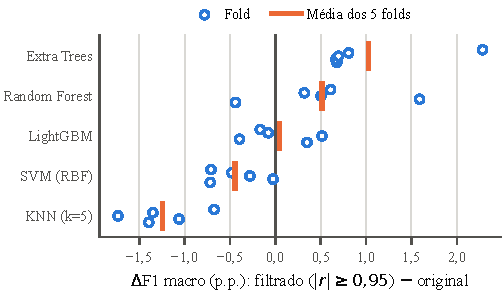
\includegraphics[width=\columnwidth]{figuras/comparacao_f1.pdf}
\caption{Diferença de F1 macro entre a condição filtrada e a original em cada \textit{fold} (círculos) e sua média (barra). Valores positivos indicam ganho com a filtragem.}
\label{fig:deltas}
\end{figure}

\begin{table}[!htb]
\centering
\caption{Diferença pareada de F1 macro (filtrado $-$ original; média $\pm$ desvio padrão entre \textit{folds}), número de \textit{folds} com ganho e tempos médios de treinamento por \textit{fold} e de predição por janela.}
\label{tab:deltas}
\scriptsize
\setlength{\tabcolsep}{3pt}
\begin{tabular}{@{}lccccc@{}}
\toprule
Modelo & $\Delta$F1 (p.p.) & Ganhos & \multicolumn{2}{c}{Treino (s)} & Pred. (ms)\\
\cmidrule(lr){4-5}
 & & & Orig. & Filt. & Filt.\\
\midrule
Extra Trees & +1,03$\pm$0,71 & 5/5 & 1,3 & 1,2 & 0,077\\
Random Forest & +0,52$\pm$0,73 & 4/5 & 4,3 & 3,2 & 0,077\\
LightGBM & +0,04$\pm$0,38 & 2/5 & 17,3 & 9,8 & 0,027\\
SVM (RBF) & $-$0,44$\pm$0,30 & 0/5 & 3,1 & 2,7 & 1,033\\
KNN (k=5) & $-$1,24$\pm$0,40 & 0/5 & 0,1 & 0,1 & 0,103\\
\bottomrule
\end{tabular}

\end{table}

A filtragem reduziu o tempo de treinamento de todos os modelos de árvores: 43\% no LightGBM (de 17,3~s para 9,8~s por \textit{fold}), 25\% no Random Forest e 8\% no Extra Trees. O tempo de predição foi inferior a 1,1~ms por janela em todos os casos, muito abaixo da duração de 2,56~s de uma janela.

\subsection{Análise por classe}
A Tabela~\ref{tab:classes} e a Fig.~\ref{fig:confusao} mostram que \textit{deitado} é a classe mais fácil (F1 de 96,2\% a 99,6\%) e que as principais confusões ocorrem entre \textit{sentado} e \textit{em pé}. Para o LightGBM, 116 janelas de \textit{sentado} foram classificadas como \textit{em pé} e 167 no sentido inverso. Essas posturas diferem pouco no movimento e principalmente na inclinação do tronco, pequena para um aparelho na cintura. Entre as atividades dinâmicas, as confusões concentram-se entre caminhar, subir e descer escadas, como também observado por Kwapisz et al.\ \cite{Kwapisz2011}.

\begin{table}[!htb]
\centering
\caption{F1 por classe (\%) na condição filtrada, calculado sobre as predições dos cinco \textit{folds}.}
\label{tab:classes}
\scriptsize
\setlength{\tabcolsep}{3pt}
\begin{tabular}{@{}lcccccc@{}}
\toprule
Modelo & Cam. & Sub. & Desc. & Sent. & Em pé & Deit.\\
\midrule
Extra Trees & 96,0 & 93,7 & 94,4 & 89,4 & 90,5 & 99,6\\
Random Forest & 95,7 & 93,7 & 93,9 & 89,4 & 90,3 & 99,6\\
LightGBM & 96,7 & 94,7 & 95,8 & 91,6 & 92,4 & 99,6\\
SVM (RBF) & 95,7 & 94,3 & 93,5 & 88,7 & 90,4 & 97,1\\
KNN (k=5) & 92,8 & 91,8 & 90,7 & 78,9 & 83,8 & 96,2\\
\bottomrule
\end{tabular}

\end{table}

\begin{figure}[!htb]
\centering
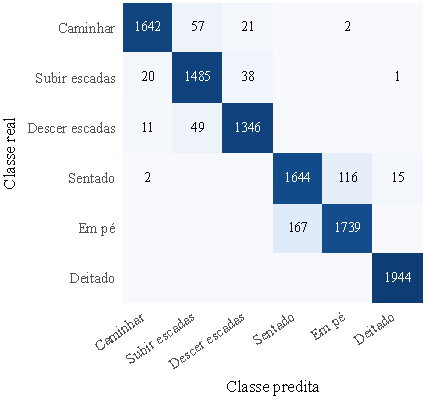
\includegraphics[width=0.92\columnwidth]{figuras/confusao_melhor.pdf}
\caption{Matriz de confusão do LightGBM com filtragem ($|r|\geq0{,}95$), somando as predições dos cinco \textit{folds} (10\,299 janelas).}
\label{fig:confusao}
\end{figure}

As perdas do KNN com a filtragem concentram-se justamente nas posturas estáticas: o F1 caiu de 82,2\% para 78,9\% em \textit{sentado}, de 85,8\% para 83,8\% em \textit{em pé} e de 98,5\% para 96,2\% em \textit{deitado}, enquanto as atividades dinâmicas variaram menos de 0,6 p.p. No SVM, a maior queda também ocorreu em \textit{deitado} (de 98,2\% para 97,1\%). No Extra Trees, os ganhos apareceram principalmente em caminhar (+1,7 p.p.) e descer escadas (+1,9 p.p.).

\subsection{Sensibilidade ao limiar}
A Fig.~\ref{fig:sensibilidade} mostra que os três modelos de árvores mantêm o F1 macro praticamente constante entre os limiares 0,99 e 0,80. O LightGBM variou apenas entre 94,89\% e 95,15\%, e o Random Forest obteve 94,09\% com $\tau=0{,}80$, usando somente 98 atributos (72\% a menos que o conjunto original). Nesse limiar, o tempo de treinamento do LightGBM caiu para 5,2~s, 70\% abaixo da condição sem filtro. O SVM e o KNN, por outro lado, perdem desempenho à medida que o limiar diminui: o SVM passa de 93,68\% sem filtro para 92,33\% com $\tau=0{,}80$, e o KNN de 90,33\% para 88,61\%.

\begin{figure}[!htb]
\centering
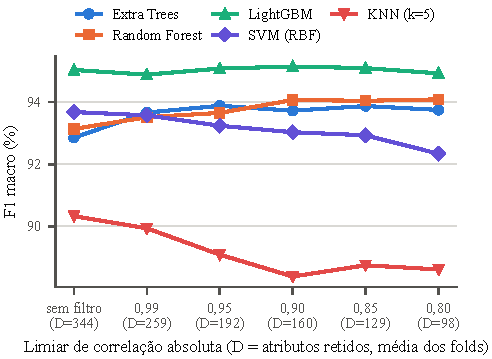
\includegraphics[width=\columnwidth]{figuras/sensibilidade_limiar.pdf}
\caption{F1 macro médio dos cinco \textit{folds} em função do limiar de correlação. $D$ indica o número médio de atributos retidos.}
\label{fig:sensibilidade}
\end{figure}

\subsection{Interpretação}
A hipótese inicial era que os métodos baseados em distância se beneficiariam mais da remoção de redundância. Os resultados mostram o contrário. Uma explicação compatível com os dados é que, após a padronização, cada atributo tem o mesmo peso na distância euclidiana; assim, várias cópias aproximadas de uma informação funcionam como um peso implícito maior para ela. No conjunto original, a orientação do aparelho em relação à gravidade aparece em vários atributos correlacionados (médias, medianas e percentis da aceleração total e ângulo de inclinação). Ao manter apenas um representante de cada grupo, o filtro reduz o peso relativo dessa informação, justamente a mais útil para separar as posturas estáticas. Além disso, atributos com $|r|$ entre 0,95 e 0,99 não são idênticos, e suas pequenas diferenças podem ajudar a definir as vizinhanças. Essa interpretação não foi isolada experimentalmente e é apresentada como hipótese.

Nos modelos de árvores, cada nó considera um subconjunto aleatório de $\sqrt{D}$ atributos. Quando muitos candidatos são cópias da mesma informação, a diversidade efetiva das divisões diminui. Remover a redundância aumenta a chance de que atributos complementares, como assimetria, entropia e frequência de pico, sejam considerados, o que é coerente com o ganho consistente do Extra Trees, cujo sorteio de limiares torna cada divisão mais dependente dos candidatos disponíveis. O LightGBM avalia todos os atributos em cada divisão e, portanto, escolhe o melhor representante de cada grupo correlacionado, com ou sem filtro. Esse comportamento está de acordo com a robustez de modelos de árvores a atributos pouco informativos observada por Grinsztajn et al.\ \cite{Grinsztajn2022} e com a seleção implícita de atributos discutida por Kotsiantis \cite{Kotsiantis2007}.

Em relação à literatura, Anguita et al.\ \cite{Anguita2013} relatam acurácia de cerca de 96\% com SVM e 561 atributos na divisão oficial da base. A melhor acurácia obtida aqui (95,2\% com LightGBM) é próxima, mas a comparação não é direta: os atributos, os classificadores e o protocolo diferem, e a validação em cinco \textit{folds} testa todos os 30 participantes, e não apenas os 9 da partição oficial de teste. A diferença de mais de 5 p.p. entre o melhor e o pior \textit{fold} de um mesmo modelo reforça a recomendação de Hammerla e Plötz \cite{Hammerla2015} de avaliar por participante e relatar a dispersão.

\section{Conclusão}
\label{sec:conclusao}
Este trabalho avaliou o efeito da filtragem de atributos por correlação de Pearson em cinco classificadores clássicos para o reconhecimento de atividades humanas na base UCI-HAR, com validação cruzada agrupada por participante. O filtro com limiar de 0,95 reduziu os atributos de 344 para cerca de 192 (44,3\%), com seleção estável entre \textit{folds}. O LightGBM obteve o maior F1 macro (aproximadamente 95,1\%) nas duas condições, e a filtragem reduziu seu tempo de treinamento em 43\% sem perda de desempenho. O Extra Trees e o Random Forest tiveram pequenos ganhos (+1,03 e +0,52 p.p.), enquanto o SVM e o KNN tiveram perdas consistentes ($-$0,44 e $-$1,24 p.p.), concentradas nas posturas estáticas.

Os objetivos propostos foram atingidos: o \textit{pipeline} foi implementado e disponibilizado \cite{Repositorio}, os cinco classificadores foram comparados nas duas condições, a sensibilidade ao limiar foi analisada e a redução de custo foi medida. A hipótese de que os métodos baseados em distância seriam os mais beneficiados não foi confirmada. A filtragem por correlação mostrou-se adequada para reduzir o custo de comitês de árvores, mas deve ser verificada caso a caso em SVM e KNN.

Entre as limitações, destacam-se o uso de uma única base, com 30 participantes e sensor sempre na cintura; os hiperparâmetros fixos, que podem favorecer uma das condições; o pequeno número de \textit{folds}, que não permite testes estatísticos com poder adequado; e a medição de tempo em computador pessoal, e não em dispositivo embarcado. A explicação proposta para a queda de SVM e KNN também não foi testada diretamente.

Como trabalhos futuros, sugerem-se: ajustar os hiperparâmetros por validação interna agrupada em cada condição; repetir a validação com outras partições para estimar melhor a incerteza; testar a hipótese do peso implícito, comparando a filtragem com ponderação ou seleção supervisionada de atributos; avaliar outras bases, como a HAR70+, voltada a idosos \cite{HAR70}; e medir latência, memória e energia em um dispositivo embarcado.

\section*{Disponibilidade do código}
O código-fonte, os resultados por \textit{fold}, as predições e os arquivos deste artigo estão disponíveis publicamente em \url{https://github.com/IEigenheer/fho-ia-har-classicos} \cite{Repositorio}.


\balance
\bibliographystyle{IEEEtran}
\bibliography{referencias}

\end{document}
